\documentclass[fleqn]{article}
\usepackage[nodisplayskipstretch]{setspace}
\usepackage{amsmath, nccmath, bm}
\usepackage{amssymb}
\usepackage{enumitem}
\usepackage{etoolbox}
\usepackage[normalem]{ulem}
\usepackage[hidelinks,colorlinks=true,urlcolor=blue,linkcolor=black]{hyperref}
\usepackage{graphicx}
\usepackage{float}
\usepackage{changepage}
\usepackage{environ,capt-of}
\usepackage{matlab-prettifier}

\let\oldfigure\figure% Store original figure float environment
\let\endoldfigure\endfigure
\RenewEnviron{figure}[1][H]{% Update figure environment
  %\par\vspace{\intextsep}% Assume in-text placement, so insert appropriate vertical spacing
  \noindent
  % \patchcmd{<cmd>}{<search>}{<replace>}{<success>}{<failure>}
  \patchcmd{\BODY}{\caption}{\captionof{figure}}{}{}% Replace \caption with \captionof{figure} inside \BODY
  % Set "figure"
  \begin{minipage}{\linewidth}
    \BODY
  \end{minipage}
  %\par\vspace{\intextsep}% Assume in-text placement, so insert appropriate vertical spacing
}

\makeatletter
\begingroup
  \catcode`\$=6 %
  \catcode`\#=12 %
  \gdef\href@split$1#$2#$3\\$4{%
    \hyper@@link{$1}{$2}{\uline{$4}}% or \underline
    \endgroup
  }%
\endgroup

\newcommand{\zerodisplayskip}{
	\setlength{\abovedisplayskip}{0pt}%
	\setlength{\belowdisplayskip}{0pt}%
	\setlength{\abovedisplayshortskip}{0pt}%
	\setlength{\belowdisplayshortskip}{0pt}%
	\setlength{\mathindent}{0pt}}
	
\title{Homework 4}
\author{Owen Sowatzke}
\date{March 29, 2024}

\begin{document}

	\offinterlineskip
	\setlength{\lineskip}{12pt}
	\zerodisplayskip
	\maketitle
	
	\begin{enumerate}
		\item Show that if the activation function of the hidden layer is linear, a three layer network is equivalent to a two layer one.
		
		\begin{figure}[H]
			\centerline{\fbox{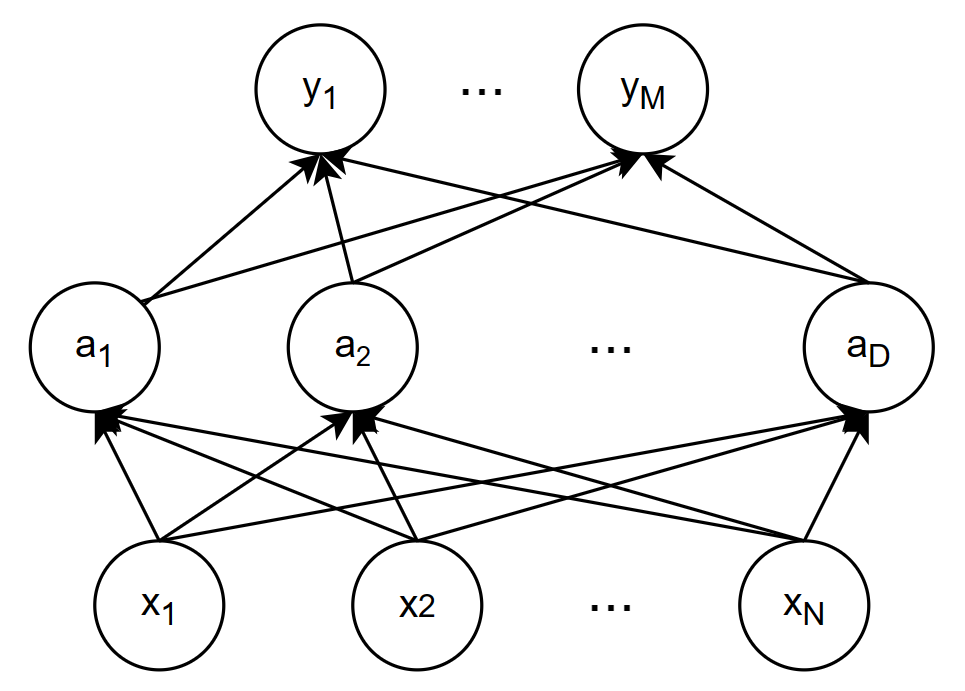
\includegraphics[width=0.4\textwidth]{neural_network_3_layer.png}}}
			\caption{3-Layer Neural Network}
			\label{neural_network_3_layer}
		\end{figure}
	
		The output of the neural network is given by:
		
		$\mathbf{y} = Q_2(\mathbf{A_2}Q_1(\mathbf{A_1}\mathbf{x} + \mathbf{b_1}) + \mathbf{b_2})$
		
		where $Q_1(\boldsymbol{\alpha})$ is the activation function of the hidden layer.
		
		If $Q_1(\boldsymbol{\alpha})$ is linear, it can be rewritten as $\mathbf{A_3}\boldsymbol{\alpha} + \mathbf{b_3}$. 
		
		$\Rightarrow Q_1(\mathbf{A_1}\mathbf{x} + \mathbf{b_1}) = \mathbf{A_3}(\mathbf{A_1}\mathbf{x} + \mathbf{b_1}) + \mathbf{b_3} = \mathbf{A_3}\mathbf{A_1}\mathbf{x} + \mathbf{A_3}\mathbf{b_1} + \mathbf{b_3}$
		
		Let $\mathbf{A_4} = \mathbf{A_3}\mathbf{A_1}$ and $\mathbf{b_4} = \mathbf{A_3}\mathbf{b_1} + \mathbf{b_3}$
		
		$\Rightarrow Q_1(\mathbf{A_1}\mathbf{x} + \mathbf{b_1}) = \mathbf{A_4}\mathbf{x} + \mathbf{b_4}$
		
		$\therefore$ the output of the neural network is given by:
		
		$\mathbf{y} = Q_2(\mathbf{A_2}(\mathbf{A_4}\mathbf{x} + \mathbf{b_4}) + \mathbf{b_2})) = Q_2(\mathbf{A_2}\mathbf{A_4}\mathbf{x} + \mathbf{A_2}\mathbf{b_4} + \mathbf{b_2})$
		
		Let $\mathbf{A} = \mathbf{A_2}\mathbf{A_4}$ and $\mathbf{b} = \mathbf{A_2}\mathbf{b_4} + \mathbf{b_2}$
		
		$\Rightarrow \mathbf{y} = Q_2(\mathbf{A}\mathbf{x} + \mathbf{b})$
		
		Note that $\mathbf{A}$ is a matrix and $\mathbf{b}$ is a vector. Therefore, a three layer neural network with a linear activation function for its hidden layer is equivalent to two-layer neural network.
		
		\begin{figure}[H]
			\centerline{\fbox{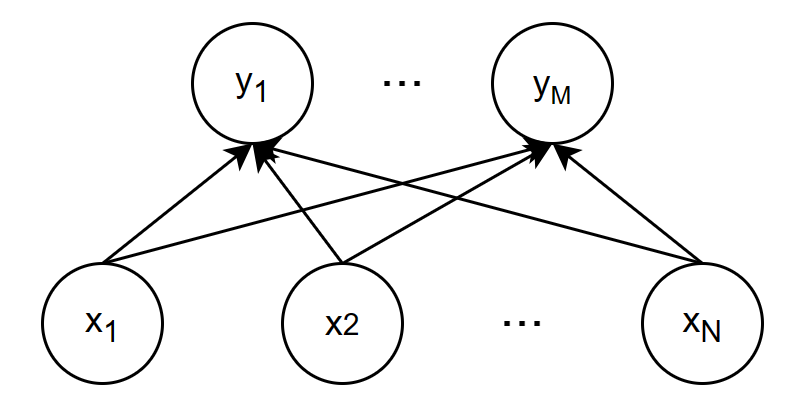
\includegraphics[width=0.4\textwidth]{neural_network_2_layer.png}}}
			\caption{2-Layer Neural Network}
			\label{neural_network_2_layer}
		\end{figure}
		
		\item Assume that a network produces the output $y_i$ in response to the i-th training image from class 1, and the output $x_i$ in response to the i-th training image from class 2. We wish to train the network to maximize the cost function $J(\text{net}) = \frac{\sum_{i}^{N}{y_i^2}}{\sum_{i}^{N}{x_i^2}}$. Derive the gradient for this cost function and describe how the network updates might be made using batch training and a single image at a time.
		
		We can re-express the cost function in matrix-vector notation as follows:
		
		\begin{equation*}
			J(\text{net}) = \frac{\mathbf{y}^T\mathbf{y}}{\mathbf{x}^T\mathbf{x}}
		\end{equation*}
		
		where $\mathbf{x} = \begin{bmatrix}x_1 & x_2 & \cdots & x_N \end{bmatrix}^T$ and $\mathbf{y} = \begin{bmatrix}y_1 & y_2 & \cdots & y_N \end{bmatrix}^T$
		
		Solving for the gradient of $J$ with respect to $\mathbf{x}$ and $\mathbf{y}$, we get the following: 
		
		\begin{equation*}
			\nabla_{\mathbf{y}}{J} = \frac{2\mathbf{y}}{\mathbf{x}^T\mathbf{x}} \ \text{and}\ \nabla_{\mathbf{x}}{J} = -\frac{2\mathbf{x}\mathbf{y}^T\mathbf{y}}{(\mathbf{x}^T\mathbf{x})^2}
		\end{equation*}		
		
		Define $\mathbf{z} = \begin{bmatrix} \mathbf{y} \\ \mathbf{x} \end{bmatrix}$. Then, we can express $\nabla_{\mathbf{z}}{J}$ as follows:
		
		\begin{equation*}
			\nabla_{\mathbf{z}}{J} = \begin{bmatrix}
				\frac{2\mathbf{y}}{\mathbf{x}^T\mathbf{x}} \\[3pt]
				-\frac{2\mathbf{x}\mathbf{y}^T\mathbf{y}}{(\mathbf{x}^T\mathbf{x})^2}
			\end{bmatrix}
		\end{equation*}
		
		\begin{equation*}
			\Rightarrow \frac{\partial{J}}{\partial{y_i}} = \frac{2y_i}{\sum_{j=1}^{N}x_j^2}\ \text{and}\ \frac{\partial{J}}{\partial{x_i}} = -\frac{2x_i\sum_{j=1}^{N}y_j^2}{\left(\sum_{j=1}^{N}x_j^2\right)^2}
		\end{equation*}
		
		In each of the above expressions, the partial derivative of $J$ with respect to $y_i$ is dependent on $x_i$. Similarly, the partial derivative of $J$ with respect to $x_i$ is dependent on $y_i$. Since $x_i$ are $y_i$ are outputs from different training images, we are limited to batch training with samples from both classes.
		
		However, we can instead choose to maximize $\text{log}(J)$, which will implicitly maximize $J$. We can express $\text{log}(J)$ as follows:
		
		\begin{equation*}
			\text{log}(J) = \text{log}\left(\frac{\mathbf{y}^T\mathbf{y}}{\mathbf{x}^T\mathbf{x}}\right) = \text{log}(\mathbf{y}^T\mathbf{y}) - \text{log}(\mathbf{x}^T\mathbf{x})
		\end{equation*}
		
		The gradient of the $\text{log}(J)$ is given as follows:
		
		\begin{equation*}
			\nabla_{\mathbf{y}}\text{log}({J}) = \frac{2\mathbf{y}}{\mathbf{y}^T\mathbf{y}} \ \text{and}\ \nabla_{\mathbf{x}}\text{log}({J}) = -\frac{2\mathbf{x}}{\mathbf{x}^T\mathbf{x}}
		\end{equation*}
		
		Using the same expression for $\mathbf{z}$ as above, we get
		
		\begin{equation*}
			\nabla_{\mathbf{z}}{\text{log}(J)} = \begin{bmatrix}
				\frac{2\mathbf{y}}{\mathbf{y}^T\mathbf{y}} \\[3pt]
				-\frac{2\mathbf{x}}{\mathbf{x}^T\mathbf{x}}
			\end{bmatrix}
		\end{equation*}
		
		\begin{equation*}
			\Rightarrow \frac{\partial}{\partial{y_i}}\left\{\text{log}(J)\right\} = \frac{2y_i}{\sum_{j=1}^{N}y_j^2}\ \text{and}\ \frac{\partial}{\partial{x_i}}\left\{\text{log}(J)\right\} = -\frac{2x_i}{\sum_{j=1}^{N}x_j^2}
		\end{equation*}
		
		Because we are maximizing the cost function, we need to apply gradient ascent instead of gradient descent. However, we can use gradient descent and achieve the same result if we instead minimize $-\text{log}(J)$. The resulting gradients are the same as above except for a sign flip ($\frac{\partial}{\partial{y_i}}\left\{-\text{log}(J)\right\} = -\frac{\partial}{\partial{y_i}}\left\{\text{log}(J)\right\}$.)
		
		Because our gradient terms are now only a function of $x_i$ or $y_i$, we can train the neural network in separates batches for class 1 and class 2. For each $x_i$ or $y_i$ in the batch, we can compute the gradient using $\frac{\partial}{\partial{y_i}}\left\{-\text{log}(J)\right\}$ for batches of class 1 and $\frac{\partial}{\partial{y_i}}\left\{-\text{log}(J)\right\}$ for batches of class 2. Next, we average the resulting gradient. Finally, using what is called backpropagation, we apply chain rule to find partial derivatives of $-\text{log}(J)$ with respect to each intermediate term. Each of these term can then be updated using gradient descent.
		
		When training with a single sample, the gradients reduce to $\frac{\partial}{\partial{y_i}}\left\{-\text{log}(J)\right\} = -\frac{2}{y_i}$ and $\frac{\partial}{\partial{x_i}}\left\{-\text{log}(J)\right\} = \frac{2}{x_i}$. Since we only have a single sample in this case, there is no need to average the resulting gradients. We can instead simply apply backpropagation and update each of the intermediate weights.
		
		\item Using the IRIS data set available at \href{https://en.wikipedia.org/wiki/IRIS_flower_data_set}{https://en.wikipedia.org/wiki/\\IRIS\_flower\_data\_set}, design a neural network classifier. The network should have two fully connected layers. The first layer should have 2 input neurons and 5 output neurons. The second layer should have 5 input neurons and 3 outputs neurons. For each input, the output should be a 3 element vector with "1" for the correct class, and "0" corresponding to the other two classes. You may use 40 samples from each class for training, and test with the remaining. Use the ReLu function as the nonlinearity between the layers.
		
		For the computer exercise, the neural network required only 2 of the 4 features. Therefore, I had to chose 2 features from the input dataset. I chose features 3 and 4 because they resulted in better classification accuracy.
		
		\begin{enumerate}
			\item[1)] Tabulate the results in terms of classification accuracy
			
			\begin{figure}[H]
				\centerline{\fbox{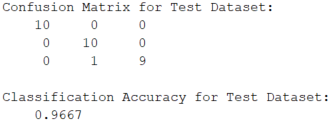
\includegraphics[width=0.8\textwidth]{test_data_results.png}}}
				\caption{Test Data Results Output by Function}
				\label{test_data_results}
			\end{figure}
		
			Referring to the figure above, the classification accuracy for the test data was 96.67\%.
			
			\item[2)] What are the number of parameters that the network must learn? How does that compare to the amount of training data?
			
			The network must learn a $2 \times 5$ matrix plus a $5 \times 1$ bias for the first fully connected layer and a $5 \times 3$ matrix plus a $3 \times 1$ bias for the second fully connected layer. Thus, the network must learn a total of 33 parameters. This is as significant number of parameters given the size of the training data set (120). Specifically, the number of learnable parameters is 27.5\% the size of the training data set. 
			
			\item[3)] How accurate is the training process, and how does it compare to the test results?
			
			\begin{figure}[H]
				\centerline{\fbox{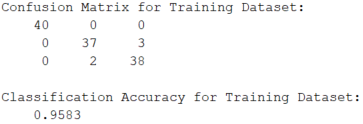
\includegraphics[width=0.8\textwidth]{training_data_results.png}}}
				\caption{Training Data Results Output by Function}
				\label{training_data_results}
			\end{figure}
		
			Referring to the figure above, the classification accuracy for the training data was 95.83\%. This is roughly the same as the test data set, which implies that the training data set is representative of the test data set. The slight performance decrease for the training data set is most likely due to the random selection of training data.
			
		\end{enumerate}
		
		Submit your code along with your answers.
		
		The code for this problem is included in Appendix \ref{neural_network} and as a separate file with the submission.
		
	\end{enumerate}
	
	\pagebreak
	\appendix
	\section{Neural Network}
	\label{neural_network}
	\lstset{style=Matlab-editor,basicstyle=\ttfamily\footnotesize}
	\lstinputlisting{Homework4_Sowatzke.m}
	\raggedbottom
	\pagebreak
\end{document}